\subsection{Anforderungsanalyse}
\label{sec:anforderungsanalyse}

Die Anforderungsanalyse bildet die Grundlage für den Architekturentwurf des CrawlDataTransformer. Die Anforderungen werden aus dem bestehenden System- und Datenkontext, den 
technischen Rahmenbedingungen, informellen Abstimmungen mit relevanten Stakeholdern sowie der wissenschaftlichen Zielsetzung der Arbeit abgeleitet. Berücksichtigt werden damit 
fachliche, technische und administrative Perspektiven auf die Transformation und ihre spätere Evaluation.

Abschnitt~4.1.1 untersucht zunächst die Einbettung des Prototyps in die bestehende Systemlandschaft sowie die Eigenschaften der Quelldaten und des vorgegebenen Zielschemas. 
Darauf aufbauend werden in Abschnitt~4.1.2 die funktionalen und nicht-funktionalen Anforderungen, technischen Vorgaben und Abgrenzungen des Prototyps formuliert. Diese 
Ergebnisse werden in Abschnitt~4.2 zu Architekturzielen und konkreten Entwurfsentscheidungen verdichtet.

\subsubsection{Analyse der Quelldaten und des Zielschemas}

Der CrawlDataTransformer ist zwischen den bestehenden Crawling-Prozessen und dem nachgelagerten Zielsystem eingeordnet. Abbildung~\ref{fig:system-context-transformation} 
zeigt diese Einbettung auf Ebene der Systemgrenzen. Die vorgelagerten Prozesse stellen Rohdatenobjekte aus Produktseiten bereit, während der CrawlDataTransformer für 
die Transformation mit der externen Gemini API kommuniziert und die erzeugten Produktobjekte über die Ziel-API an das nachgelagerte System übergibt. Die Ziel-API bildet 
die ausschließliche Schnittstelle zur produktiven Datenhaltung. Ein direkter Schreibzugriff auf deren Datenbank ist nicht vorgesehen.

\begin{figure}[H]
    \centering
    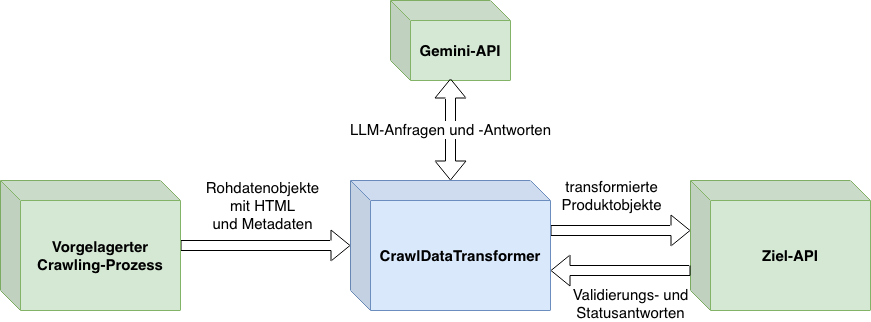
\includegraphics[width=\textwidth]{figures/Kontextsicht.png}
    \caption{Systemkontext des CrawlDataTransformer}
    \label{fig:system-context-transformation}
\end{figure}

Die Eingabedaten liegen als Rohdatenobjekte vor, die neben dem HTML-Inhalt der Produktseite technische Metadaten wie eine Kennung, die Quell-URL, einen Zeitstempel, die 
Shop-Zuordnung und Bildinformationen enthalten können. Ein gekürztes Beispiel ist in Abschnitt~A.1 dargestellt. Für die fachliche Transformation bildet insbesondere der 
HTML-Inhalt die relevante Informationsquelle. Dieser enthält jedoch neben den Produktinformationen auch Navigationselemente, Skripte, Styles, Layoutstrukturen und weitere 
Bestandteile, die für die Extraktion nicht unmittelbar relevant sind.

Die fachlichen Informationen besitzen keine einheitliche Position oder Darstellung. Produktbezeichnungen, Marken- und Herstellerangaben, Zutaten, Nährwerte, Produktgruppen 
und Verpackungsgrößen können sowohl in strukturierten HTML-Elementen als auch in frei formuliertem Text auftreten. Mengenangaben unterscheiden sich zudem hinsichtlich 
Schreibweise, Einheit und Granularität. Bei der Bestimmung der Verpackungsgröße müssen beispielsweise tatsächliche Inhaltsangaben von Grundpreisen, Nährwertreferenzen, 
Portionsgrößen und weiteren konkurrierenden Mengenangaben unterschieden werden. Die Quelldaten enthalten somit grundsätzlich die benötigten Informationen, stellen diese 
jedoch nicht in einer unmittelbar übertragbaren Struktur bereit.

Demgegenüber verlangt das Zielsystem ein fest definiertes, verschachteltes und typisiertes JSON-LD-Objekt. Ein Beispiel der Zielstruktur ist in Abschnitt~A.2 dargestellt. 
Das Schema umfasst einfache Produktattribute ebenso wie komplexe Teilobjekte, Beziehungen und typisierte Einheiten. Die erzeugten Daten müssen daher nicht nur inhaltlich 
zugeordnet, sondern auch hinsichtlich Datentypen, Objektstruktur und Einheiten konsistent abgebildet werden. Das externe Zielschema bestimmt dabei, welche fachlichen 
Informationen aus den Quelldaten hervorgehen müssen. Die konkrete Überführung eines internen Extraktionsergebnisses in das vollständige Zielobjekt erfolgt erst vor der 
Übergabe an die Ziel-API.

Zwischen den heterogenen Rohdaten und dem vorgegebenen Zielmodell besteht folglich eine Transformationslücke. Eine direkte Übernahme der Quelldaten ist weder aufgrund der 
enthaltenen Störinformationen noch aufgrund ihrer uneinheitlichen Struktur möglich. Daraus ergeben sich Anforderungen an die Vorverarbeitung, die strukturierte Extraktion, 
die Prüfung und Vereinheitlichung der Ergebnisse sowie die kontrollierte Übergabe an das Zielsystem. Diese Anforderungen werden im folgenden Abschnitt konkretisiert.

\subsubsection{Funktionale und nicht-funktionale Anforderungen}

Aus der Analyse der Quell- und Zielstrukturen, den technischen Rahmenbedingungen, den informellen Stakeholder-Abstimmungen und dem wissenschaftlichen Vergleichsziel werden 
die Anforderungen an den Prototyp abgeleitet. Die funktionalen Anforderungen beschreiben die erforderlichen Systemleistungen, während die nicht-funktionalen Anforderungen 
die maßgeblichen Qualitätseigenschaften festlegen. Die Priorisierung unterscheidet zwischen für das Forschungsziel erforderlichen Muss-Anforderungen und ergänzenden Soll-Anforderungen.

\begin{table}[H]
    \centering
    \footnotesize
    \setlength{\tabcolsep}{4pt}
    \renewcommand{\arraystretch}{1.08}
    \begin{tabular}{
        |p{0.06\textwidth}
        |p{0.73\textwidth}
        |p{0.11\textwidth}|
    }
        \hline
        \textbf{ID} &
        \textbf{Funktionale Anforderung} &
        \textbf{Priorität} \\
        \hline

        F1 &
        Der Prototyp muss mindestens ein Rohdatenobjekt mit Quellinformationen und HTML-Inhalt als Transformationsbatch entgegennehmen können. &
        Muss \\
        \hline

        F2 &
        Das HTML muss konservativ vorverarbeitet werden, sodass technisch irrelevante Bestandteile reduziert und potenziell relevante Produktinformationen erhalten bleiben. &
        Muss \\
        \hline

        F3 &
        Aus dem vorverarbeiteten Produktkontext muss ein strukturiertes internes Produktextraktionsergebnis erzeugt werden. &
        Muss \\
        \hline

        F4 &
        Die LLM-Verarbeitung muss batchbasiert und zeitlich getrennt ausführbar sein. Bearbeitungszustand und externe Batchreferenz müssen zwischen Einreichung und Ergebnisabruf erhalten bleiben. &
        Muss \\
        \hline

        F5 &
        Extraktionsergebnisse müssen gegen das interne Schema geprüft und unterschiedliche Mengen-, Einheiten- und Textdarstellungen normalisiert werden. &
        Muss \\
        \hline

        F6 &
        Für das Referenzdatenfeld \textit{ProductSizing} muss aus derselben vorverarbeiteten Eingabe eine getrennte regelbasierte Vorhersage erzeugt werden. &
        Muss \\
        \hline

        F7 &
        Normalisierte Produktdaten sollen mit lokal verfügbaren Produktdaten abgeglichen werden können. Bei uneindeutigen Ergebnissen darf eine semantische Unterstützung eingesetzt werden. &
        Soll \\
        \hline

        F8 &
        Das interne Produktergebnis muss auf das externe Zielmodell abgebildet und ausschließlich über die Ziel-API übergeben werden. &
        Muss \\
        \hline

        F9 &
        LLM-basierte und regelbasierte Ergebnisse müssen derselben Ground Truth gegenübergestellt und auf Request- sowie Batch-Ebene ausgewertet werden können. &
        Muss \\
        \hline

        F10 &
        Eingaben, Zwischenstände, Statusinformationen, Fehler und Ergebnisse müssen schrittweise gespeichert werden, damit zeitlich unterbrochene Verarbeitungsphasen fortgesetzt werden können. &
        Muss \\
        \hline
    \end{tabular}
    \caption{Funktionale Anforderungen an den CrawlDataTransformer}
    \label{tab:functional-requirements}
\end{table}

Die funktionalen Anforderungen folgen dem Datenfluss von der Eingabe bis zur Übergabe an das Zielsystem. Die regelbasierte Verarbeitung ist dabei auf \textit{ProductSizing} begrenzt 
und stellt keine vollständige Alternative zur LLM-basierten Produktextraktion dar. Sie dient als feldspezifische Baseline für den in F9 geforderten Vergleich.

\begin{table}[H]
    \centering
    \footnotesize
    \setlength{\tabcolsep}{4pt}
    \renewcommand{\arraystretch}{1.08}
    \begin{tabular}{
        |p{0.06\textwidth}
        |p{0.73\textwidth}
        |p{0.11\textwidth}|
    }
        \hline
        \textbf{ID} &
        \textbf{Nicht-funktionale Anforderung} &
        \textbf{Priorität} \\
        \hline

        N1 &
        Nur strukturell verarbeitbare Ergebnisse dürfen an nachgelagerte Verarbeitungsschritte und die Ziel-API übergeben werden. &
        Muss \\
        \hline

        N2 &
        Der Fehler einer einzelnen Transformationsanfrage darf die Weiterverarbeitung anderer Anfragen desselben Batches nicht grundsätzlich verhindern. &
        Muss \\
        \hline

        N3 &
        Eingaben, Zwischenergebnisse, externe Antworten, Zustandsübergänge und Fehler müssen einer konkreten Transformationsanfrage zugeordnet werden können. &
        Muss \\
        \hline

        N4 &
        Die Ergebnisse beider Extraktionsansätze müssen getrennt gespeichert und unter gemeinsamen Vergleichsbedingungen evaluierbar sein. &
        Muss \\
        \hline

        N5 &
        Fachliche Verarbeitungsschritte und technische Integrationen müssen klar abgegrenzt und unabhängig anpassbar sein. &
        Muss \\
        \hline

        N6 &
        Tokenverbrauch, LLM-Kosten und lokale Verarbeitungslaufzeiten müssen erfasst und für die spätere Auswertung bereitgestellt werden. &
        Muss \\
        \hline
    \end{tabular}
    \caption{Nicht-funktionale Anforderungen an den CrawlDataTransformer}
    \label{tab:non-functional-requirements}
\end{table}

Der technische Gestaltungsraum wird durch den bestehenden Projektkontext begrenzt. Der Prototyp wird in Python umgesetzt und verwendet die Gemini API für die LLM-basierte Extraktion 
sowie die optionale semantische Unterstützung des Produkt-Matchings. Die lokale MongoDB dient ausschließlich als Arbeits-, Transformations- und Evaluationsdatenbank. Die produktive 
Übergabe erfolgt über die Ziel-API. Das vorgelagerte Crawling-System und das externe Zielschema werden nicht verändert. Ebenso sind das Training eines eigenen Sprachmodells, ein 
vollständiger regelbasierter Ersatz der Produktextraktion sowie Anforderungen an Hochverfügbarkeit und horizontale Skalierung nicht Bestandteil der Arbeit.

Zwingend erforderlich sind damit insbesondere die Vorverarbeitung, die LLM-basierte und regelbasierte Extraktion, die zeitlich getrennte Batch-Verarbeitung, Schema-Validierung, 
Normalisierung, Persistenz, Evaluation, Fehlerisolation und Übergabe über die Ziel-API. Das semantisch unterstützte Produkt-Matching und zusätzliche Eingabekanäle erhöhen die 
praktische Nutzbarkeit, sind für den grundlegenden Vergleich der Extraktionsansätze jedoch nachgeordnet. Die Anforderungen bilden die Grundlage für die im folgenden Abschnitt 
abgeleiteten Architekturziele und Entwurfsentscheidungen.